\documentclass[10pt]{article}
\usepackage{../pplmanual}
%%% Commonly Needed packages
\usepackage{graphicx,color,calc}
\usepackage{fancyvrb}
\usepackage{makeidx}
\usepackage{alltt}
\usepackage[linkbordercolor=(0 0 1),citebordercolor=(0 1 0)]{hyperref}
%%\usepackage{xspace} <- creates problems with other hyperlink packages like "html"

%%% Commands for uniform looks of C++, Charm++, and Projections
\newcommand{\CC}{C\hbox{++}}
\newcommand{\emCC}{C\hbox{\em++}}
\newcommand{\charmpp}{\textsc{Charm++}}
\newcommand{\charmc}{\texttt{charmc}}
\newcommand{\projections}{\textsc{Projections}}
\newcommand{\converse}{\textsc{Converse}}
\newcommand{\ampi}{\textsc{AMPI}}
\newcommand{\tempo}{\textsc{TeMPO}}
\newcommand{\irecv}{\textsl{iRecv}}
\newcommand{\sdag}{\textsl{Structured Dagger}}
\newcommand{\jade}{Jade}

%%% Commands to produce margin symbols
\newcommand{\new}{\marginpar{\fbox{\bf$\mathcal{NEW}$}}}
\newcommand{\important}{\marginpar{\fbox{\bf\Huge !}}}
\newcommand{\experimental}{\marginpar{\fbox{\bf\Huge $\beta$}}}

%%% Commands for manual elements
\newcommand{\zap}[1]{ }
\newcommand{\function}[1]{{\noindent{\textsf{#1}}\\}}
\newcommand{\cmd}[1]{{\noindent{\textsf{#1}}\\}}
\newcommand{\args}[1]{\hspace*{2em}{\texttt{#1}}\\}
\newcommand{\prototype}[1]{\vspace{0.2in}\index{#1}}
\newcommand{\param}[1]{{\texttt{#1}}}
\newcommand{\kw}[1]{{\textsf{#1}\index{#1}}}
\newcommand{\uw}[1]{{\textsl{#1}}}
\newcommand{\desc}[1]{\indent{#1}}
\newcommand{\note}[1]{(\textbf{Note:} #1)}
\newcommand{\term}[1]{{\bf #1}\index{#1}}

\makeindex


\makeindex

\title{\charmpp\\ Finite Element Framework\\ Manual}
\version{1.0}
\credits{
Initial version of \charmpp{} Finite Element Framework was developed
by Milind Bhandarkar with inputs from Timothy Hinrichs and Kathikeyan
Mahesh. The current version is almost completely rewritten by
Orion Lawlor.
}

\begin{document}

\maketitle

\section{Motivation}

The Finite Element Method (FEM) approach is used in many engineering
applications with irregular domains, from elastic deformation problems to
crack propagation to fluid flow.  \charmpp{} is a free message-passing parallel
runtime system for machines from clusters of workstations to tightly-coupled
SMPs.  The \charmpp{} FEM framework allows you to write a parallel FEM program,
in C or Fortran 90, that closely resembles a serial version but includes
a few framework calls.

Using the FEM framework also allows you to take advantage of all the
features of \charmpp, including run-time load balancing,  performance
monitoring and visualization, and checkpoint/restart, with no additional
effort. The FEM framework also combines naturally with other \charmpp
frameworks built on TCHARM.


\section{Introduction/Terminology}

A FEM program manipulates elements and nodes. An element is a portion of
the problem domain, typically in the shape of a triangle, square, or hexagon
in 2D; or tetrahedron or rectangular solid in 3D.  A node is a point in the
domain.  An element knows which nodes surround it via the connectivity
table, which lists adjacent nodes.

\begin{figure}[h]
\begin{center}
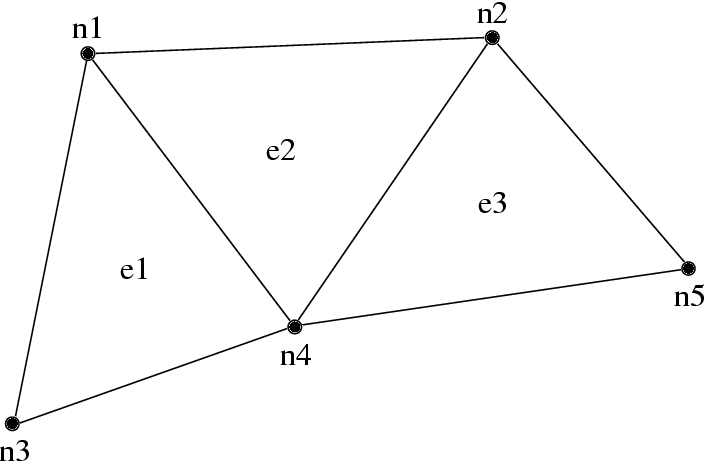
\includegraphics[width=4in]{simple_mesh}
\end{center}
\caption{3-element, 5 node mesh.}
\label{fig:simplemesh}
\end{figure}

\begin{table}[h]
\begin{center}
\begin{tabular}{||l||r|r|r||}\hline
Element & \multicolumn{3}{c||}{Adjacent Nodes} \\\hline
e1 & n1 & n3 & n4 \\
e2 & n1 & n2 & n4 \\
e3 & n2 & n4 & n5 \\
\hline
\end{tabular}
\end{center}
\caption{Connectivity table for mesh in figure~\ref{fig:simplemesh}.}
\label{table:simplemesh}
\end{table}

A typical FEM program performs some element-by-element calculations which
update adjacent node values; then some node-by-node calculations.  For
example, a material dynamics program has the structure:

\begin{alltt}
     time loop
          element loop-- Element deformation applies forces to
          surrounding nodes
          node loop-- Forces and boundary conditions change node
          positions
     end time loop
\end{alltt}

We can parallelize such FEM programs by partitioning the serial mesh
elements into several chunks  (at least one chunk per processor; perhaps
even more).  During partitioning, we give nodes and elements new,
chunk-local numbers.  Below, we partition the mesh above into two chunks, A
and B.

\begin{figure}[h]
\begin{center}
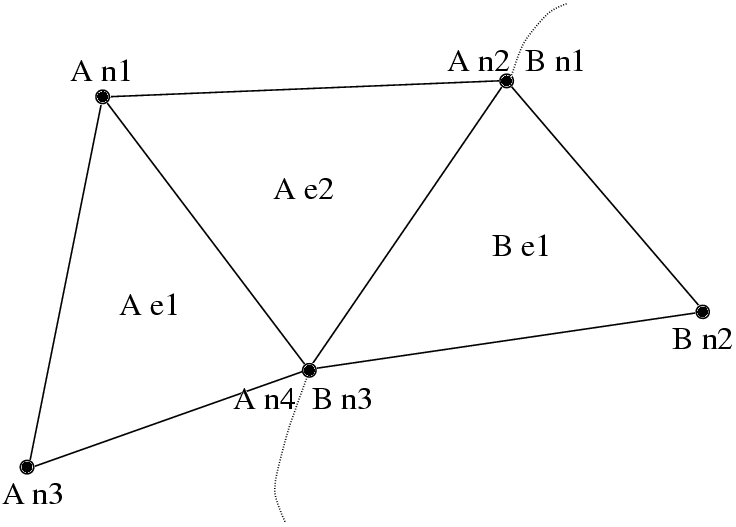
\includegraphics[width=4in]{partitioned_mesh}
\end{center}
\caption{Partitioned mesh.}
\label{fig:partitionedmesh}
\end{figure}

\begin{table}[h]
\begin{center}
\begin{tabular}{||l||r|r|r||}\hline
Element & \multicolumn{3}{c||}{Adjacent Nodes} \\\hline
e1 & n1 & n3 & n4 \\
e2 & n1 & n2 & n4 \\
\hline
\end{tabular}
\end{center}
\caption{Connectivity table for chunk A in figure~\ref{fig:partitionedmesh}.}
\label{table:chunkA}
\end{table}

\begin{table}[h]
\begin{center}
\begin{tabular}{||l||r|r|r||}\hline
Element & \multicolumn{3}{c||}{Adjacent Nodes}\\\hline
e1 & n1 & n2 & n3 \\
\hline
\end{tabular}
\end{center}
\caption{Connectivity table for chunk B in figure~\ref{fig:partitionedmesh}.}
\label{table:chunkB}
\end{table}

Note that chunk A's node n2 and B's node n1 were actually the same node in
the original mesh-- partitioning split this single node into two shared
copies (one on each chunk).  However, since adding forces is associative, we
can handle shared nodes by computing the forces normally (ignoring the
existence of the other chunk), then adding both chunks' net force for the
shared node together.  This ``node update'' will give us the same resulting
force on each shared node as we would get without partitioning, thus the
same positions, thus the same final result.  Hence, each chunk's time loop
has the structure:

\begin{alltt}
     chunk time loop
          element loop-- Element deformation applies forces to
          surrounding nodes
          <update forces on shared nodes>
          node loop-- Forces and boundary conditions change node
          positions
     end time loop
\end{alltt}

This is exactly the form of the time loop for a \charmpp{} FEM framework
program.  The framework will accept a serial mesh, partition it, distribute
the chunks to each processor, allow the user to run their time loop, and
handle the node-updates.


\section{Structure of a FEM Framework Program}

A FEM framework program consists of three subroutines: \kw{init()}, \kw{driver()},
and \kw{mesh\_updated()}.  \kw{init()} and \kw{mesh\_updated()} are called by the FEM framework
only on the first processor -- these routines typically do specialized I/O,
startup and shutdown tasks.  \kw{driver()} is called for every chunk on every
processor, and does the main work of the program.  In the language of the
TCHARM manual, \kw{init()} and \kw{mesh\_updated()} run in the serial context, 
and \kw{driver()} runs in the parallel context.


\begin{alltt}
     subroutine init
          read the serial mesh and configuration data
     end subroutine

     subroutine driver
          get local mesh chunk
          time loop
               FEM computations
               update shared node fields
               more FEM computations
          end time loop
     end subroutine

     subroutine mesh_updated
          write out results; possibly modify serial mesh
     end subroutine
\end{alltt}

\section{Compilation and Execution}

A FEM framework program is a \charmpp\ program, so you must begin by
downloading the latest source version of \charmpp\ from
{\tt http://charm.cs.uiuc.edu/}.  Build the source with 
{\tt ./build FEM version} or {\tt cd} into the build directory, 
{\tt version/tmp}, and type {\tt make FEM}.
To compile a FEM program, pass the {\tt -language fem} (for C) or 
{\tt -language femf} (for Fortran) option to {\tt charmc}.

In a charm installation, see charm/version/pgms/charm++/fem/
for several example and test programs.

At runtime, an FEM framework program accepts the following
options, in addition to all the usual Charm++ options described in 
the Charm++ "Installation and Usage Manual".

\begin{itemize}
\item {\tt +vp} $v$  

Create $v$ mesh chunks, or ``virtual processors''.
By default, the number of mesh chunks is equal to the number of 
physical processors (set with {\tt +p} $p$).


\item {\tt +write}

Skip \kw{driver()}.
After running \kw{init()} normally, the framework partitions the mesh, 
writes the mesh partitions to files, and exits.  As usual, the
{\tt +vp} $v$ option controls the number of mesh partitions.


\item {\tt +read}

Skip \kw{init()}.
The framework reads the partitioned input mesh from files
and calls \kw{driver()}.  Together with {\tt +write}, this option
allows you to separate out the mesh preparation and partitioning 
phase from the actual parallel solution run.

This can be useful, for example, if \kw{init()} requires more memory 
to hold the unpartitioned mesh than is available on one processor of 
the parallel machine.  To avoid this limitation, you can run the program
with {\tt +write} on a machine with a lot of memory to prepare the input
files, then copy the files and run with {\tt +read} on a machine with 
a lot of processors.

{\tt +read} can also be useful during debugging or performance tuning, 
by skipping the (potentially slow) mesh preparation phase.


\item {\tt +tcharm\_trace fem}

Give a diagnostic printout on every call into the FEM framework.
This can be useful for locating a sudden crash, or understanding
how the program and framework interact.  Because printing the 
diagnostics can slow a program down, use this option with care.

\end{itemize}


\section{FEM Framework API Reference}

Some of the routines in the FEM framework have different requirements or meanings
depending on where they are called from.  When a routine is described
as being "called from driver", this means it is called in the parallel
context---from \kw{driver()} itself, any subroutine called by \kw{driver()},
or from whatever routine is runs the FEM-attached TCHARM threads.
When a routine is described as being "called from init", this means it is 
called in the serial context---from \kw{init()} itself, from any subroutine
called from \kw{init()}, or from whatever TCHARM code executes before the
\kw{FEM\_Attach}.


\subsection{Utility}

\prototype{FEM\_Num\_partitions}
\function{int FEM\_Num\_partitions();}
\function{function integer :: FEM\_Num\_partitions()}

     Return the number of mesh chunks in the current computation.  Can
     only be called from the driver routine.

\prototype{FEM\_My\_partitions}
\function{int FEM\_My\_partition();}
\function{function integer :: FEM\_My\_partition()}

     Return the number of the current chunk, from 0 to
     \kw{num\_partitions}-1.  Can only be called from the driver routine.

\prototype{FEM\_Timer}
\function{double FEM\_Timer();}
\function{function double precision :: FEM\_Timer()}

     Return the current wall clock time, in seconds.  Resolution is
     machine-dependent, but is at worst 10ms.

\prototype{FEM\_Print\_partition}
\function{void FEM\_Print\_partition();}
\function{subroutine FEM\_Print\_partition()}

     Print a debugging representation of the current chunk's mesh.
     Prints the entire connectivity array, and data associated with
     each local node and element.

\prototype{FEM\_Print}
\function{void FEM\_Print(const char *str);}
\function{subroutine FEM\_Print(str)}
\args{  character*, intent(in) :: str}

     Print the given string.  Works on all machines; unlike \kw{printf} or
     \kw{print *}, which may not work on all parallel machines.

\section{Mesh}

These routines describe and retreive the finite element mesh for this
computation.  A mesh, from the framework's perspective, is a list of
elements and nodes, together with uninterpreted data associated with each.
Elements map to nodes via the connectivity table for that element type.
Elements and nodes have both a global number (number in
the serial mesh) as well as a chunk-local number (number in the partitioned
mesh chunk).  The FEM framework currently uses the package Metis to do 
partitioning.

A simple program would set the serial mesh in init, get the partitioned
chunk in driver, and work on that chunk.  A more complex program would set
the initial mesh in init; then get, work on, update and repartition the mesh
several times in driver via \kw{FEM\_Update\_mesh}.

From \kw{init()}, the \kw{FEM\_Set\_} routines describe the serial mesh, which
will be partitioned into chunks.

From \kw{driver()}, the \kw{FEM\_Get\_} routines ask for the current mesh
chunk; the \kw{FEM\_Set\_} routines describe a new partitioned mesh chunk.  The
new chunk need not have the same number of elements or nodes as the old chunk;
but any new added nodes are assumed private (not shared).
\kw{FEM\_Update\_mesh} will reassemble a serial version of the mesh from the
new pieces and optionally repartition the serial mesh.

From \kw{mesh\_updated()}, the \kw{FEM\_Get} and \kw{FEM\_Set} routines
manipulate the serial mesh.   \kw{mesh\_updated()} is only executed if you call
\kw{FEM\_Update\_mesh} during driver-- otherwise, \kw{mesh\_updated()} can be an
empty procedure.  The parameter \kw{callMeshUpdated} is passed down to
\kw{mesh\_updated()}.

\prototype{FEM\_Set\_mesh}
\function{void FEM\_Set\_mesh(int nElem, int nNodes, int nodePerEl,const int* conn);}

     This is a convenience routine equivalent to:
\begin{alltt}
          FEM\_Set\_node(nNodes,0);
          FEM\_Set\_elem(0,nElem,0,nodePerEl);
          FEM\_Set\_elem\_Conn(0,conn);
\end{alltt}

\function{subroutine FEM\_Set\_mesh(nElem,nNodes,nodePerEl,conn)}
    \args{integer, intent(in) :: nElem, nNodes, nodePerEl}
    \args{integer, intent(in), dimension(nElem,nodePerEl) :: conn;}

     This is a convenience routine equivalent to:
\begin{alltt}
          CALL FEM\_Set\_node(nNodes,0)
          CALL FEM\_Set\_elem(1,nElem,0,nodePerEl)
          CALL FEM\_Set\_elem\_Conn\_c(1,conn)
\end{alltt}

\prototype{FEM\_Get/Set\_elem}
\function{void FEM\_Set\_elem(int elType,int  nEl,int  doublePerEl,int  nodePerEl);}
\function{void FEM\_Get\_elem(int elType,int *nEl,int *doublePerEl,int *nodePerEl);}
\function{subroutine FEM\_Set\_elem(elType,nEl,doublePerEl,nodePerEl)}
  \args{integer, intent(in)  :: elType,nEl,doublePerEl,nodePerEl}
\function{subroutine FEM\_Get\_elem(elType,nEl,doublePerEl,nodePerEl)}
  \args{integer, intent(in)  :: elType}
  \args{integer, intent(out) :: nEl,doublePerEl,nodePerEl}

     Describe/retreive the number and type of elements.  \kw{ElType} is the
number of element types registered so far (the first element type is 1, then 2,
etc.).  \kw{nEl} is the number of elements being registered.  \kw{doublesPerEl}
and \kw{nodePerEl} are the number of doubles of user data, and nodes (respectively) associated with each element.
		
     \kw{doublePerEl} or \kw{nodePerEl} may be zero, indicating that no user
data or connectivity data (respectively) is associated with the element.

     You can make this and any other mesh setup calls in any order---there is no need 
to make them in linearly increasing order.  However, for a given type of element
\kw{FEM\_Set\_elem} must be called before setting that element's connectivity or data.


\prototype{FEM\_Get/Set\_elem\_conn}
\function{void FEM\_Set\_elem\_conn(int elType,const int *conn);}
\function{void FEM\_Get\_elem\_conn(int elType,int *conn);}
\function{subroutine FEM\_Set\_elem\_conn\_r(elType,conn)}
  \args{integer, intent(in)  :: elType}
  \args{integer, intent(in),  dimension(nodePerEl,nEl) :: conn}
\function{subroutine FEM\_Get\_elem\_conn\_r(elType,conn)}
  \args{integer, intent(in)  :: elType}
  \args{integer, intent(out), dimension(nodePerEl,nEl) :: conn}
\function{subroutine FEM\_Set\_elem\_conn\_c(elType,conn)}
  \args{integer, intent(in)  :: elType}
  \args{integer, intent(in),  dimension(nEl,nodePerEl) :: conn}
\function{subroutine FEM\_Get\_elem\_conn\_c(elType,conn)}
  \args{integer, intent(in)  :: elType}
  \args{integer, intent(out), dimension(nEl,nodePerEl) :: conn}

     Describe/retreive the element connectivity array for this element
     type.  The connectivity array is indexed by the element number,
     and gives the indices of the nodes surrounding the element.  It is
     hence \kw{nodePerEl*nEl} integers long.

     The C version array indices are zero-based, and must be stored in
     row-major order (a given element's surrounding nodes are stored
     contiguously in the conn array).  The Fortran version indices are
     one-based, and are available in row-major (named \_r) and
     column-major (named \_c) versions.  We recommend row-major storage
     because it results in better cache utilization (because the nodes
     around an element are stored contiguously).
     

\prototype{FEM\_Get/Set\_node}
\function{void FEM\_Set\_node(int  nNode,int  doublePerNode);}
\function{void FEM\_Get\_node(int *nNode,int *doublePerNode);}
\function{subroutine FEM\_Set\_node(nNode,doublePerNode)}
  \args{integer, intent(in)  :: nNode,doublePerNode}
\function{subroutine FEM\_Get\_node(nNode,doublePerNode)}
  \args{integer, intent(out) :: nNode,doublePerNode}

     Describe/retreive the number of nodes and doubles of user data
     associated with each node.  There is only one type of node, so no
     \kw{nodeType} identifier is needed.

     \kw{doublePerNode} may be zero, indicating that no user data is
     associated with each node.

\prototype{FEM\_Get/Set\_data}
\function{void FEM\_Set\_node\_data(const double *data);}
\function{void FEM\_Get\_node\_data(double *data);}
\function{void FEM\_Set\_elem\_data(int elType,const double *data);}
\function{void FEM\_Get\_elem\_data(int elType,double *data);}
\function{subroutine FEM\_Set\_node\_data\_r(data)}
  \args{REAL*8, intent(in),  dimension(doublePerNode,nNode)  :: data}
\function{subroutine FEM\_Get\_node\_data\_r(data)}
  \args{REAL*8, intent(out), dimension(doublePerNode,nNode)  :: data}
\function{subroutine FEM\_Set\_node\_data\_c(data)}
  \args{REAL*8, intent(in),  dimension(nNode,doublePerNode)  :: data}
\function{subroutine FEM\_Get\_node\_data\_c(data)}
  \args{REAL*8, intent(out), dimension(nNode,doublePerNode)  :: data}

\function{subroutine FEM\_Set\_elem\_data\_r(elType,data)}
  \args{integer, intent(in)  :: elType}
  \args{REAL*8, intent(in),  dimension(doublePerElem,nElem)  :: data}
\function{subroutine FEM\_Get\_elem\_data\_r(elType,data)}
  \args{integer, intent(in)  :: elType}
  \args{REAL*8, intent(out), dimension(doublePerElem,nElem)  :: data}
\function{subroutine FEM\_Set\_elem\_data\_c(elType,data)}
  \args{integer, intent(in)  :: elType}
  \args{REAL*8, intent(in),  dimension(nElem,doublePerElem)  :: data}
\function{subroutine FEM\_Get\_elem\_data\_c(elType,data)}
  \args{integer, intent(in)  :: elType}
  \args{REAL*8, intent(out), dimension(nElem,doublePerElem)  :: data}

     Describe/retrieve the optional, uninterpreted user data associated with
each node and element.  This user data is partitioned and reassembled along
with the connectivity matrix, and may include initial conditions, node locations,
material types, or any other data needed or produced by the program.   The Fortran
arrays can be row- or column- major (see \kw{FEM\_Set\_elem\_conn} for
details).  The row-major form is preferred.


\prototype{FEM\_Set\_sparse}
\function{void FEM\_Set\_sparse(int S\_id,int nRec,
         const int *nodes,int nodesPerRec,
         const void *data,int dataPerRec,int dataType);}
\function{subroutine FEM\_Set\_sparse(S\_id,nRec,nodes,nodesPerRec,data,dataPerRec,dataType)}
  \args{integer, intent(in) :: S\_id,nRec,nodesPerRec,dataPerRec,dataType}
  \args{integer, intent(in) :: nodes(nodesPerRec,nRec)}
  \args{varies,  intent(in) :: data(dataPerRec,nRec)}

Register \kw{nRec} sparse data records with the framework under the number \kw{S\_id}. 
The first call to \kw{FEM\_Set\_sparse} must give a \kw{S\_id} of zero in C (1 in fortran);
and subsequent calls to \kw{FEM\_Set\_sparse} must give increasing consecutive \kw{S\_id}s.

One sparse data record consists of some number of nodes, listed in the
\kw{nodes} array, and some amount of user data, listed in the data array.
Sparse data records are copied into the chunks that contains all that record's listed 
nodes.  Sparse data records are normally used to describe mesh boundary conditions--
for node-associated boundary conditions, \kw{nodesPerRec} is 1; for triangle-associated
boundary conditions, \kw{nodesPerRec} is 3.

In general, \kw{nodePerRec} gives the number of nodes associated with each
sparse data record, and \kw{nodes} gives the actual node numbers.
\kw{dataPerRec} gives the number of data items associated with each sparse 
data record, and \kw{dataType}, one of \kw{FEM\_BYTE}, \kw{FEM\_INT},
\kw{FEM\_REAL}, or \kw{FEM\_DOUBLE}, gives the type of each data item.
As usual, you may change or delete the \kw{nodes} and \kw{data} arrays after this
call returns.

For example, if the first set of sparse data is 17 sparse data records, each 
containing 2 nodes stored in \kw{bNodes} and 3 integers stored in \kw{bDesc}, 
we would make the call:
\begin{alltt}
/*C version*/
  FEM_Set_sparse(0,17, bNodes,2, bDesc,3,FEM_INT);
! Fortran version
  CALL FEM_Set_sparse(1,17, bNodes,2, bDesc,3,FEM_INT)
\end{alltt}

\prototype{FEM\_Set\_sparse\_elem}
\function{void FEM\_Set\_sparse\_elem(int S\_id,const int *rec2elem);}
\function{subroutine FEM\_Set\_sparse\_elem(S\_id,rec2elem)}
  \args{integer, intent(in) :: S\_id}
  \args{integer, intent(in) :: rec2elem(2,nRec)}

Attach the previously-set sparse records \kw{S\_id} to the given elements.
\kw{rec2elem} consists of pairs of integers---one for each sparse data record.
The first integer in the pair is the
element type to attach the sparse record to, and the second integer
gives the element number within that type.  For example, to attach
the 3 sparse records at \kw{S\_id} to the elements numbered 10, 11, and 12
of the element type \kw{elType}, use:

\begin{alltt}
/*C version*/
  int rec2elem[]={elType,10, elType,11, elType,12};
  FEM_Set_sparse_elem(S_id,rec2elem);
! Fortran version
  integer :: rec2elem(2,3);
  rec2elem(1,:)=elType
  rec2elem(2,1)=10; rec2elem(2,2)=11; rec2elem(2,3)=12;
  CALL FEM_Set_sparse_elem(S_id,rec2elem)
\end{alltt}


\prototype{FEM\_Get\_sparse}
\function{int  FEM\_Get\_sparse\_length(int S\_id);}
\function{void FEM\_Get\_sparse(int S\_id,int *nodes,void *data);}
\function{function FEM\_Get\_sparse\_length(S\_id);}
  \args{integer, intent(in) :: S\_id}
  \args{integer, intent(out) :: FEM\_Get\_sparse\_Length}
\function{subroutine FEM\_Get\_sparse(S\_id,nodes,data);}
  \args{integer, intent(in) :: S\_id}
  \args{integer, intent(out) :: nodes(nodesPerRec,FEM\_Get\_sparse\_Length(S\_id))}
  \args{varies,  intent(out) :: data(dataPerRec,FEM\_Get\_sparse\_Length(S\_id))}

Retrieve the previously registered sparse data from the framework.
\kw{FEM\_Get\_sparse\_length} returns the number of records of sparse
data registered under the given \kw{S\_id}; zero indicates no records
are available.  \kw{FEM\_Get\_sparse} returns you the actual nodes
(translated to local node numbers) and unchanged user data for
these sparse records.


\subsection {Mesh Ghosts}
An option to add "ghosts" to a mesh is provided by the framework. A ghost is a local read-only copy of a node or element that actually lives on another chunk.  Ghosts are typically added to the boundary of a chunk to allow the real (non-ghost) elements at the boundary to access values across the processor boundary.  This makes a chunk ``feel'' as if it was part of a complete unpartitioned mesh.

\subsubsection{Setting up the ghost layer}
The framework's ghost handling is element-centric. You specify which kinds of elements should be ghosts and how they connect by listing their "tuples" via calls in the \kw{init()} routine.  

\begin{itemize}
\item

\prototype{FEM\_Add\_ghost\_layer}
\function{void FEM\_Add\_ghost\_layer(int nodesPerTuple,int doAddNodes);}
\function{subroutine FEM\_Add\_ghost\_layer(nodesPerTuple,doAddNodes)}
  \args{integer, intent(in) :: nodesPerTuple,doAddNodes}
This routine creates a new layer of ghosts around each FEM chunk. \kw{nodesPerTuple} is the number of shared nodes that together form a "tuple". \kw{doAddNodes} specifies that you want ghost nodes as well as elements.

A tuple is an unordered set of nodes, and is an abstract way to describe which ghosts
your application needs---an element will be added to your chunk if it connects to at 
least one of your tuples.  For example, if you have a 3D, tetrahedral element that require ghosts 
on all 4 of its sides, this is equivalent to requiring ghosts of every element that shares all 3
nodes of one of your triangular faces, so for you a tuple is a 3-node face.  If you have a 2D shape
and want edge-adjacency, for you a tuple is a 2-node edge.  If you want node-adjacent ghosts,
a tuple is a single node.

Calling this routine several times creates several layers of ghost elements, and the different layers need not have the same parameters.

\item
\prototype{FEM\_Add\_ghost\_elem}
\function{void FEM\_Add\_ghost\_elem(int elType,int tuplesPerElem,const int *elem2tuple);}
\function{subroutine FEM\_Add\_ghost\_elem(elType,tuplesPerElem,elem2tuple)}
  \args{integer, intent(in) :: elType,tuplesPerElem}
  \args{integer, intent(in) :: elem2tuple(nodesPerTuple,tuplesPerElem)}

This call is used to specify which type of element is to be added to the current ghost layer. \kw{tuplesPerElem} and \kw{elem2tuple} specify a mapping between each element and the surrounding tuples.  The \kw{elem2tuple} table lists, for each tuple, the nodes of this element which form the tuple, specified as element-local numbers---indices into this element's connectivity entry. The \kw{elem2tuple} table should have nodesPerTuple*tuplesPerElem entries, and no entry should be greater than nodePerEl for that element type.

\kw{elem2tuple} can include special indices--- -1 for C, 0 for Fortran---that indicate the
corresponding tuple is shorter than usual.  For example, if \kw{nodesPerTuple} for this layer
is 4, for 4-node quadrilateral faces, you could set one entry in \kw{elem2tuple} to -1 to specify
a 3-node triangular face.  Tuples of different lengths will never match, so this is just
a simple way to add ghosts from two kinds of tuples at once.

\end{itemize}

The above two routines are always used together. For example, if your elements are 3-node triangles and you only require one shared node for inclusion in a single ghost layer, you would use:
\begin{alltt}
   FEM\_Add\_ghost\_layer(1,0); /* 1 node per tuple */
   const static int tri2node[]={0,1,2};
   FEM\_Add\_ghost\_elem(0,3,tri2node); /* triangles are surrounded by 3 nodes */
\end{alltt}

If you require two shared nodes (a shared edge), the code will look like:
\begin{alltt}    
   FEM\_Add\_ghost\_layer(2,0); /* 2 nodes per tuple */
   const static int tri2edge[]={0,1,  1,2,  2,0};
   FEM\_Add\_ghost\_elem(0,3,tri2edge); /*triangles are surrounded by 3 edges */
\end{alltt}



\subsubsection{Extracting the ghost layer}
After the ghost layer is created, we need a way to distinquish real nodes and elements 
from ghost nodes and elements. FEM\_Get\_node and FEM\_Get\_elem return the 
\textbf{total} number of nodes and elements, including ghosts. The routines below 
return the index of the first ghost node or element.

\prototype{FEM\_Get\_ghost}
\function{int FEM\_Get\_node\_ghost(void);}
\function{int FEM\_Get\_elem\_ghost(int elemType);}
The examples below iterate over the real and ghost elements.
\begin{alltt}
C version:
        int firstGhost,max;
        FEM\_Get\_node(\&max, \&ignored);
        firstGhost=FEM\_Get\_node\_ghost();
        for (i=0;i<firstGhost;i++)
                ... i is a real node...
        for (i=firstGhost;i<max;i++)
                ... i is a ghost node ...

Fortran version:
        call FEM\_Get\_node(max,ignored);
        firstGhost=FEM\_Get\_node\_ghost();
        do i=1,firstGhost-1
                ... i is a real node...
        end do
        do i=firstGhost,max
                ... i is a ghost node...
        end do
\end{alltt}

\subsubsection{Symmetries and Ghosts--Geometric Layer}

The FEM framework can create ghosts not only of things that are on other 
processors, but also for various problem symmetries, like mirror reflection,
and various types of periodicities.  The interface for these ghosts is 
simple---you ask for the symmetries to be created, then you will get 
extra ghosts along each symmetry boundary.  The symmetry ghosts are
updated properly during any communication, even if the symmetry ghosts
are ghosts of real local elements.


\prototype{FEM\_Add\_linear\_periodicity}
\function{void FEM\_Add\_linear\_periodicity(
        int nFaces,int nPer,
        const int *facesA,const int *facesB,
        int nNodes,const double *nodeLocs
        );}
\function{
SUBROUTINE FEM\_Add\_linear\_periodicity(nFaces,nPer,facesA,facesB,
                                nNodes,nodeLocs)}
  \args{integer, intent(in) :: nFaces, nPer, nNodes}
  \args{integer, intent(in) :: facesA(nPer,nFaces), facesB(nPer,nFaces)}
  \args{double precision, intent(in) :: nodeLocs(3,nNodes)}

Make facesA and facesB match up under linear translation.
Each face of facesA must match up with exactly one face of
facesB, but both the faces and the nodes within a face can be
permuted in any order---the order is recovered by matching 3d locations
in the nodeLocs array.

This call can be repeated, for example if the domain is periodic along several
directions.  This call can only be issued from \kw{init()}.



\prototype{FEM\_Sym\_coordinates}
\function{void FEM\_Sym\_coordinates(int elTypeOrMinusOne,double *locs);}
\function{SUBROUTINE FEM\_Sym\_coordinates(elTypeOrZero,locs)}
  \args{integer, intent(in) :: elTypeOrZero}
  \args{double precision, intent(inout) :: locs(3,<number of items>)}

This call adjusts the 3d locations listed in \kw{locs} so they respect the symmetries
of their corresponding item.  If elTypeOrZero is an element type,
the locations are adjusted to match with the corresponding element;
if elTypeOrZero is zero, the locations are adjusted to match up with
the corresponding node.

This call is needed because symmetry ghost nodes and elements
initially have their original locations, which must be adjusted
to respect the symmetry boundaries.  Thus this call is needed
both for initial location data (e.g., from \kw{FEM\_Get\_node\_data})
as well as any communicated location data (e.g., from
\kw{FEM\_Update\_ghost\_field}).

This call can only be issued from \kw{driver()}.



\subsubsection{Symmetries and Ghosts--Lower Layer}

The geometric symmetry layer in the preceeding section is actually
a thin wrapper around this lower, more difficult to use layer.

\prototype{FEM\_Set\_sym\_nodes}
\function{void FEM\_Set\_sym\_nodes(const int *canon,const int *sym);}
\function{SUBROUTINE FEM\_Set\_sym\_nodes(canon,sym)}
  \args{integer, intent(in) :: canon(nNodes)}
  \args{integer, intent(in) :: sym(nNodes)}

This call describes all possible symmetries in an extremely terse format.
It can only be called from \kw{init()}.
The ``canonicalization array'' canon maps nodes to their canonical 
representative---if canon($i$)=canon($j$), nodes $i$ and $j$ are 
images of each other under some symmetry.  The sym array has bits set
for each symmetry boundary passing through a node.

For example, a 2d domain with 6 elements A, B, C, D, E, and F and 12 
nodes numbered 1-12 that is 
mirror-symmetric on the horizontal boundaries but periodic in the 
vertical boundaries would look like:

\begin{alltt}
   D^'|  D^ |  E^ |  F^ |  F^`
   -  1  -  2  -  3  -  4  -
   A' |  A  |  B  |  C  |  C`
   -  5  -  6  -  7  -  8  -
   D' |  D  |  E  |  F  |  F`
   -  9  - 10  -  11 -  12 -
   Av'|  Av |  Bv |  Cv |  Cv`

  v indicates the value has been shifted down (bottom boundary),
  ^ indicates the value has been shifted up (top boundary),
  ' indicates the value has been copied from the left (right boundary),
  ` indicates the value has been copied from the right (left boundary).
\end{alltt}

If we mark the left border with 1, the top with 2, the right with 4,
and the bottom with 8, this situation is indicated by topologically pasting the 
top row to the bottom row by setting their \kw{canon} entries equal, and 
marking each node with its symmetries.

\begin{center}
\begin{tabular}{|l|l|l|}\hline
  Node & \kw{canon} &  \kw{sym}              \\\hline
    1  &    1  &      3 (left + top)   \\
    2  &    2  &      2 (top)   \\
    3  &    3  &      2 (top)   \\
    4  &    4  &      6 (top + right)   \\
    5  &    5  &      1 (left)   \\
    6  &    6  &      0 (none)   \\
    7  &    7  &      0 (none)   \\
    8  &    8  &      4 (right)   \\
    9  &    1  &      9 (left+bottom)    \\
    10 &    2  &      8 (bottom)   \\
    11 &    3  &      8 (bottom)   \\
    12 &    4  &      12 (bottom+right)   \\
\hline
\end{tabular}
\end{center}


\prototype{FEM\_Get\_sym}
\function{void FEM\_Get\_sym(int elTypeOrMinusOne,int *destSym);}
\function{void FEM\_Get\_sym(elTypeOrZero,destSym);}
  \args{integer, intent(in) :: elTypeOrMinusOne }
  \args{integer, intent(out) :: destSym(nItems)}

This call extracts the list of symmetry conditions that apply to 
an item type.  If elType is an element type, it returns the
symmetry conditions that apply to that element type; if elType is
-1 (zero for Fortran), it returns the symmetry conditions that apply
to the nodes.  Symmetry conditions are normally only nonzero
for ghost nodes and elements.


Mirror symmetry conditions are not yet supported, nor are
multiple layers of symmetry ghosts.  

% FIXME: document these
% void FEM_Set_partition(int *elem2chunk)
% int FTN_NAME(FEM_GET_COMM_PARTNERS,fem_get_comm_partners)(void)
% int FTN_NAME(FEM_GET_COMM_PARTNER,fem_get_comm_partner)(int *partnerNo)
% int FTN_NAME(FEM_GET_COMM_COUNT,fem_get_comm_count)(int *partnerNo)
% void FTN_NAME(FEM_GET_COMM_NODES,fem_get_comm_nodes)(int *pNo,int *nodeNos)
% void FTN_NAME(FEM_GET_ELEM_NUMBERS,fem_get_elem_numbers)(int *gNo)
% void fem_get_node_numbers(int *gNo)


\subsection{Mesh Modification}

\prototype{FEM\_Add\_node}
\function{void FEM\_Add\_node(int localIdx,int nBetween,int *betweenNodes);}
\function{subroutine FEM\_Add\_node(localIdx,nBetween,betweenNodes)}
    \args{integer, intent(in) :: localIdx,nBetween}
    \args{integer, intent(in) :: betweenNodes(nBetween)}

This call adds a new node, with local index \kw{localIdx}, to the current mesh chunk. 
BetweenNodes lists the local node numbers of the all the nodes the new node is 
"between"-- for example, when adding a new node along an edge, nBetween is 2
and betweenNodes lists the endpoints of the edge.
\kw{FEM\_Add\_node} only affects the current chunk-- no other chunks are affected.

To create shared nodes, \kw{FEM\_Add\_node} must be called on all the chunks that 
share the node, to create the local copies of the node.
When adding multiple nodes, \kw{FEM\_Add\_node} must be called in the same order 
on all the processors that share the new node--that is, if two new
nodes $x$ and $y$ are added between chunks $a$ and $b$, if $a$ calls
\kw{FEM\_Add\_node} with its local number for $x$ before it calls \kw{FEM\_Add\_node}
with its local number for $y$, $b$ must also add its copy of node $x$ before $y$.


\prototype{FEM\_Update\_mesh}
\function{void FEM\_Update\_mesh(int callMeshUpdated,int doWhat);}
\function{subroutine FEM\_Update\_mesh(callMeshUpdated,doWhat)}
    \args{integer, intent(in) :: callMeshUpdated,doWhat}

Reassemble the mesh chunks from each partition into a single serial mesh.
Can only be called from driver; and must be called by the driver routine for
every chunk. \kw{FEM\_Get} calls from
\kw{driver()} will only return the new mesh after a \kw{FEM\_Update\_mesh} call
where \kw{doWhat} is 1; otherwise \kw{FEM\_Get} returns the old mesh.

If \kw{callMeshUpdated} is not zero, \kw{mesh\_updated(callMeshUpdated)}
will be called on the first processor after the mesh is reassembled.

%     If \kw{doRepartition} is 0, the mesh is not repartitioned, and \kw{FEM\_Update\_mesh}
%returns immediately.  If \kw{doRepartition} is 1, \kw{FEM\_Update\_mesh} blocks
%until the reassembled serial mesh is repartitioned back into chunks and redistributed.
%If \kw{doRepartition} is 2, 

\begin{center}
\begin{tabular}{|l|l|l|l|}\hline
\kw{doWhat} & Repartition? & \kw{FEM\_Update\_mesh} \\\hline
0 & No & Immediately continues execution \\
1 & Yes & Blocks for the new partition \\
2 & No & Blocks until \kw{mesh\_updated()} is complete\\
\hline
\end{tabular}
\end{center}

For example, \kw{FEM\_Update\_mesh}(k,0) reassembles the mesh and calls
\kw{mesh\_updated(k)} while the driver routines continue with the computation.
This might be useful, for example, for writing out intermediate solutions as a 
single file; writing outputs from \kw{driver()} is more efficient but often results 
in a separate file for each mesh chunk.

   To block the driver routines during the call to \kw{mesh\_updated(k)}, such as 
at the end of the computation when the drivers have no other work to do, 
use \kw{FEM\_Update\_mesh}(k,2).

     To reassemble, modify, and repartition the mesh, use \kw{FEM\_Update\_mesh}(k,1).
It may be easier to perform major mesh modifications from \kw{mesh\_updated(k)} than
the drivers, since the entire serial mesh is available to \kw{mesh\_updated(k)}.

     \kw{FEM\_Update\_mesh} reassembles the serial mesh with an attempt to
     preserve the element and node global numbering.  If the new mesh
     has the same number and type of elements and nodes, the global
     numbers (and hence serial mesh) will be unchanged.  If new
     elements or nodes are added at each chunk, they will be assigned
     new unique global numbers.  If elements or nodes are removed,
     their global numbers are not re-used-- you can detect the
     resulting holes in the serial mesh since the user data associated
     with the deleted elements will be all zero.  Generally, however, it
     is less error-prone to perform mesh modifications only in \kw{driver()}
     or only in \kw{mesh\_updated(k)}, rather than some in both.



\section{Communication Fields}

The FEM framework handles the updating of the values of shared nodes-- that
is, it combines shared nodes' values across all processors.  The basic
mechanism to do this update is the field-- numeric data items associated
with each node. We make no assumptions about the meaning of the node data,
and allow various data types and non-communicated data associated with each
node.  To do this, the framework must be able to find the data items
associated with each node in memory.

Each field represents a (set of) node data items stored in a contiguous array,
indexed by node number.  You create a field once, with \kw{FEM\_Create\_field},
then pass the resulting field ID to \kw{FEM\_Update\_field} (which does the
shared node communication) and/or \kw{FEM\_Reduce\_field} (which applies a
reduction over node values).

\prototype{FEM\_Create\_simple\_field}
\function{int FEM\_Create\_simple\_field(int base\_type,int rec\_len);}
\function{function integer :: FEM\_Create\_simple\_field(base\_type, rec\_len)}
  \args{integer, intent(in)  :: base\_type, rec\_len}
    
    Creates and returns a FEM field ID, which can be passed to
\kw{FEM\_Update\_field} and \kw{FEM\_Reduce\_field.}  Can only be called from
\kw{driver()}.  A field is a range of values stored in your array that the framework
can access.  For example, a field that describes data associated with each local 
node can be used by \kw{FEM\_Update\_field} to find and update the values of 
shared nodes.

    \kw{base\_type} describes the kind of data item associated with each
record, one of:

     \begin{itemize}
        \item \kw{FEM\_BYTE}-- unsigned char, INTEGER*1, or CHARACTER*1
        \item \kw{FEM\_INT}-- int or INTEGER*4
        \item \kw{FEM\_REAL}-- float or REAL*4
        \item \kw{FEM\_DOUBLE}-- double, DOUBLE PRECISION, or REAL*8
     \end{itemize}

     \kw{rec\_len} describes the number of data items associated with each
record, an integer at least 1.

     For example, if you store a 3D force for each node \kw{n}, in an array
indexed by 3*\kw{n}, \kw{base\_type} is \kw{FEM\_DOUBLE} and \kw{rec\_len} is 3.
You can register this node force for update with:

\begin{alltt}
          /* C */
          double *nodeForce; ... allocated as 3*n_nodes...
          int Fid=FEM_Create_simple_field(FEM_DOUBLE,3);
 
          ! - Fortran90
          REAL*8 ALLOCATABLE, dimension(:) :: nodeForce
          INTEGER :: Fid
          Fid=FEM_Create_simple_field(FEM_DOUBLE,3)
\end{alltt}



\prototype{FEM\_Create\_field}
\function{int FEM\_Create\_field(int base\_type,int rec\_len,int offset,int dist);}
\function{function integer :: FEM\_Create\_field(base\_type, rec\_len, offset, dist)}
  \args{integer, intent(in)  :: base\_type, rec\_len, offset, dist}

     A more sophisticated version of \kw{FEM\_Create\_simple\_field}, for 
when your data is padded or stored in a complex structure.

     \kw{offset} is the byte offset from the start of your array to the
first data item, a non-negative integer.  In \kw{FEM\_Create\_simple\_field},
\kw{offset} is always zero.

     \kw{dist} is the byte offset from the first record to the
second, a positive integer.  In \kw{FEM\_Create\_simple\_field}, this is
always equal to \kw{rec\_len} times the size of one item.

\begin{figure}[h]
\begin{center}
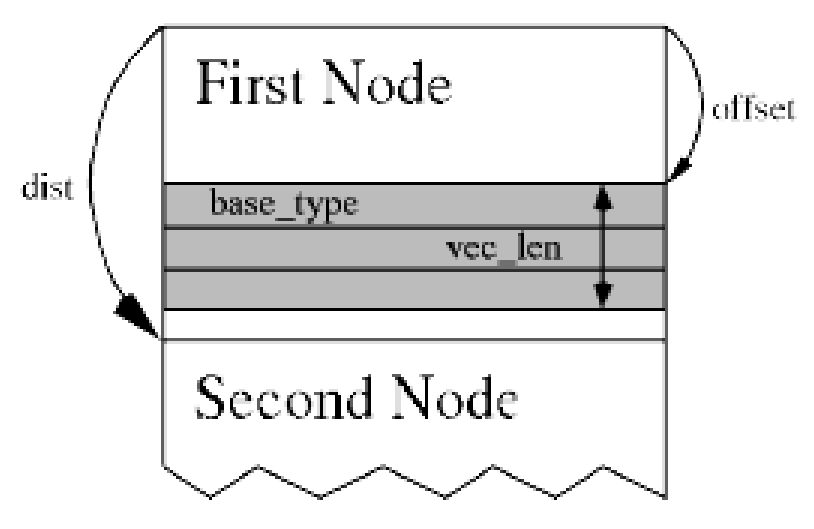
\includegraphics[width=4in]{create_field}
\end{center}
\caption{Creating a complex Node Field.}
\label{fig:createfield}
\end{figure}


If the 3D force is a member \kw{fXYZ} of a structure (in C) or named type
(in Fortran 90) \kw{node\_type}, in an array called \kw{nodes}, you can
register this node force for update with:

\begin{alltt}
          /* C */
          node_type *nodes;
          ...allocate nodes array as n_nodes...
          int Fid=FEM_Create_field(FEM_DOUBLE,3,
              (int)((char *)\&nodes[0].fXYZ-(char *)nodes),
              (int)((char *)\&nodes[1]-(char *)\&nodes[0]) );
 
          ! - Fortran90
          TYPE(node_type), ALLOCATABLE, dimension(:) :: nodes
          INTEGER :: Fid
          ...allocate nodes array as n_nodes...
          Fid=FEM_Create_field(FEM_DOUBLE,3,
              offsetof(nodes(1), nodes(1)%fXYZ),
              offsetof(nodes(1), nodes(2)) )
\end{alltt}

     This example uses the Fortran-only helper routine \kw{offsetof}, which
     returns the offset in bytes of memory between its two given
     variables.  The C version uses pointer arithmetic to achieve the
     same result.

\prototype{FEM\_Update\_field}
\function{void FEM\_Update\_field(int Fid,void *nodes);}
\function{subroutine FEM\_Update\_field(Fid,nodes)}
  \args{integer, intent(in)  :: Fid}
  \args{varies, intent(inout) :: nodes}

     Combine a field of all shared nodes with the other chunks.  Sums
     the value of the given field across all chunks that share each
     node.  For the example above, once each chunk has computed the net
     force on each local node, this routine will sum the net force
     across all shared nodes.

     \kw{FEM\_Update\_field} can only be called from driver, and to be useful,
     must be called from every chunk's driver routine.

     After this routine returns, the given field of each shared node
     will be the same across all processors that share the node.

\prototype{FEM\_Read\_field}
\function{void FEM\_Read\_field(int Fid,void *nodes,char *fName);}
\function{subroutine FEM\_Read\_field(Fid,nodes,fName)}
  \args{integer, intent(in)  :: Fid}
  \args{varies, intent(out) :: nodes}
  \args{character*, intent(in) :: fName}

     Read a field out of the given serial input file.  The serial input
     file is line-oriented ASCII-- each line begins with the global
     node number (which must match the line order in the file),
     followed by the data to be read into the node field.  The
     remainder of each line is unread.  If called from Fortran, the
     first line must be numbered 1; if called from C, the first line
     must be numbered zero.  All fields are separated by white space
     (any number of tabs or spaces).

     For example, if we have called \kw{Create\_field} to describe 3 doubles,
     the input file could begin with

\begin{alltt}
          1    0.2    0.7    -0.3      First node
          2    0.4    1.12   -17.26    another node
          ...
\end{alltt}

     \kw{FEM\_Read\_field} must be called from driver at any time, independent
     of other chunks.

\prototype{FEM\_Reduce\_field}
\function{void FEM\_Reduce\_field(int Fid,const void *nodes,void *out,int op);}
\function{subroutine FEM\_Reduce\_field(Fid,nodes,outVal,op)}
  \args{integer, intent(in)  :: Fid,op}
  \args{varies, intent(in) :: nodes}
  \args{varies, intent(out) :: outVal}

Combine a field from each node, according to op, across all chunks.
Shared nodes are not double-counted-- only once copy will contribute to the
reduction.  After \kw{Reduce\_field} returns, all chunks will have identical
values in \kw{outVal,} which must be \kw{vec\_len} copies of \kw{base\_type}.

     May only be called from driver, and to complete, must be called
     from every chunk's driver routine.

     \kw{op} must be one of:

\begin{itemize}
        \item \kw{FEM\_SUM}-- each element of \kw{outVal} will be the sum 
of the corresponding fields of all nodes
        \item \kw{FEM\_MIN}-- each element of \kw{outVal} will be the 
smallest value among the corresponding field of all nodes
        \item \kw{FEM\_MAX}-- each element of \kw{outVal} will be the largest 
value among the corresponding field of all nodes
\end{itemize}


\prototype{FEM\_Reduce}
\function{void FEM\_Reduce(int Fid,const void *inVal,void *outVal,int op);}
\function{subroutine FEM\_Reduce(Fid,inVal,outVal,op)}
  \args{integer, intent(in)  :: Fid,op}
  \args{varies, intent(in) :: inVal}
  \args{varies, intent(out) :: outVal}

     Combine a field from each chunk, acoording to \kw{op}, across all chunks.
\kw{Fid} is only used for the \kw{base\_type} and \kw{vec\_len}-- offset and
\kw{dist} are not used.  After this call returns, all chunks will have
identical values in \kw{outVal}.  Op has the same values and meaning as
\kw{FEM\_Reduce\_field}.

     May only be called from driver, and to complete, must be called
     from every chunk's driver routine.



\subsection{Ghost Communication}

It is possible to get values for a chunk's ghost nodes and elements from the neighbors. To do this, use:

\prototype{FEM\_Update\_ghost\_field}
\function{void FEM\_Update\_ghost\_field(int Fid, int elTypeOrMinusOne, void *data);}
\function{subroutine FEM\_Update\_ghost\_field(Fid,elTypeOrZero,data)}
  \args{integer, intent(in)  :: Fid,elTypeOrZero}
  \args{varies, intent(inout) :: data}

This has the same requirements and call sequence as \kw{FEM\_Update\_field}, except it applies to ghosts. You specify which type of element to exchange using the elType parameter. Specify -1 (C version) or 0 (fortran version) to exchange node values.  


\subsection{Ghost List Exchange}

It is possible to exchange sparse lists of ghost elements between FEM chunks.

\prototype{FEM\_Exchange\_ghost\_lists}
\function{void FEM\_Exchange\_ghost\_lists(int elemType,int nIdx,const int *localIdx);}
\function{subroutine FEM\_Exchange\_ghost\_lists(elemType,nIdx,localIdx)}
  \args{integer, intent(in)  :: elemType,nIdx}
  \args{integer, intent(in) :: localIdx[nIdx]}

This routine sends the local element indices in localIdx to those neighboring chunks that connect to its ghost elements on the other side.  That is, if the element
\kw{localIdx[i]} has a ghost on some chunk \kw{c}, \kw{localIdx[i]} will be sent to 
and show up in the ghost list of chunk \kw{c}.

\prototype{FEM\_Get\_ghost\_list\_length}
\function{int FEM\_Get\_ghost\_list\_length(void);}
Returns the number of entries in my ghost list---the number of my ghosts that
other chunks passed to their call to \kw{FEM\_Exchange\_ghost\_lists}.

\prototype{FEM\_Get\_ghost\_list}
\function{void FEM\_Get\_ghost\_list(int *retLocalIdx);}
\function{subroutine FEM\_Get\_ghost\_list(retLocalIdx)}
  \args{integer, intent(out) :: retLocalIdx[FEM\_Get\_ghost\_list\_length()]}

These routines access the list of local elements sent by other chunks.  
The returned indices will all refer to ghost elements in my chunk.



% Permanently undocumented (i.e., officially denied) features:
%   FEM_Serial_Split(ndom) ! Partition into ndom domains
%   FEM_Serial_Begin(idom) ! Begin accessing the idom'th domain
%   
% "There has to be a better way:"
%   FEM_Composite_elem, FEM_Combine_elem


\input{index}
\end{document}
